\section{Discussion of our results}
\label{sec:discussion}
As we outline in section~\ref{sec:results}, we are not able to reproduce all
the results from the literature in our own simulations.  Through our study of
social force models, we have come across a wide variety of different
improvements. We believe that some of these improvements will be able to solve
the discrepancies between our results and the results in \cite{self-org}.
These improvements are presented in this section.  The section is divided into
three parts: A discussion of the effects of modifying  the interaction forces,
a discussion of parameter values, and a discussion of possible errors related
to our implementation of the simulation.

\subsection{Modifying interaction forces}
\label{sec:new-forces}
An obvious possibility when discussing why we do not see the expected results,
is analysing the forces that comprise the model to see if we can identify any
reasons for the discrepancy between the results we see and those we expected.
As a starting point for this analysis, we look at additional forces presented
in other articles, but that are not included in the model we have simulated.

We speculate that the reason that we do not see the faster-is-slower effect is
that our model does not take into account frictional effect between
pedestrians.  Such a force has been suggested as a cause of the
faster-is-slower effect in \cite{HelbingNew} and a term for the frictional
force is given in \cite{helbing00}, where they reproduce the faster-is-slower
effect through simulations.

The friction force is given as a force which is perpendicular to the direction
of the repulsive force, as illustrated in  figure~\ref{fig:friction}. The
magnitude of the frictional component depends on both the distance and the
relative velocity between the two pedestrians and would make it harder for
pedestrians to move in dense crowds.

\begin{figure}[hb]
    \centering
    \begin{tikzpicture}
        \node (p1) [pedestrian] {};
        \node (p2) [pedestrian,above=0pt of p1] {};
        \node (p1 target) [point,left=1cm of p2] {};
        \node (p2 target) [point,left=1cm of p1] {};

        \draw [blue,vector] (p1.north) -- +(1.0,0);
        \draw [blue,vector] (p2.south) -- +(-1.0,0);
        \draw [red,vector] (p1.south) -- +(0,-1.0);
        \draw [red,vector] (p2.north) -- +(0,1.0);
        \draw [vector] (p1) -- (p1 target);
        \draw [vector] (p2) -- (p2 target);
    \end{tikzpicture}
    \caption[Friction forces]{Friction forces (blue) are perpendicular to the
    repulsive forces (red) between two pedestrians and make it harder for
    pedestrians to move in crowded areas.}
    \label{fig:friction}
\end{figure}

When looking at the simulations, there are two types of behaviour that we find
presents us with problems: pedestrians walking directly towards each other do
not try to avoid colliding, and pedestrians running towards a wall decelerate
at the same rate as pedestrians walking towards it. These types of behaviour
are illustrated in figure~\ref{fig:extra-forces-behaviour}.

\begin{figure}[h]
    \centering
    \subfloat[Pedestrian $\alpha$ walking towards pedestrian $\beta$.]{
        \begin{tikzpicture}
            \node (p moving) [pedestrian,
                              label=below:$\alpha$] {};
            \node (p static) [pedestrian,right=of p moving,
                              label=below:$\beta$] {};
            \node (divert) [point,above right=5mm of p static] {};
            \node (first) [point,left=5mm of p static] {};

            \draw[->,dashed,red] (p moving) -- (p static);
            \draw[->,dashed,blue] (p moving) -- (first) to[bend left] (divert) ;

            \path [use as bounding box]
                (p static) +(1.5,0) +(0,1.5)
                (p moving) +(-1.5,0) +(0,-1.5);
        \end{tikzpicture}
        \label{subfig:colliding}
        }
    \subfloat[Pedestrians moving towards a wall at different speeds.]{
        \begin{tikzpicture}
            \node (slow) [pedestrian] {};
            \node (fast) [pedestrian, right=of slow] {};

            \node (slow target) [point, above=4mm of slow] {};
            \node (fast target) [point, above=8mm of fast] {};
            \node (slow repulsion) [point, below=5mm of slow] {};
            \node (fast repulsion) [point, below=5mm of fast] {};

            \node (wall start) [wall endpoint,above left=of slow] {};
            \node (wall end) [wall endpoint,above right=of fast] {};
            \draw[wall] (wall start) -- (wall end);

            \draw[blue,vector] (slow) -- (slow target);
            \draw[blue,vector] (fast) -- (fast target);
            \draw[red,vector] (slow) -- (slow repulsion);
            \draw[red,vector] (fast) -- (fast repulsion);

            \path [use as bounding box] (wall start) +(-1,0) (wall end)
            +(1,0);
        \end{tikzpicture}
        \label{subfig:equal-repulsion}}
    \caption[Problematic behaviour]{Problematic behaviour.
    \subref{subfig:colliding} A pedestrian, $\alpha$ walking towards another
    pedestrian, $\beta$, does not divert to the side (red line), even though
    doing so would avoid a collision (blue line).
    \subref{subfig:equal-repulsion} Pedestrians heading towards the wall at
    different speeds (blue arrows) are repulsed equally (red arrows).}
    \label{fig:extra-forces-behaviour}
\end{figure}

Inspired by the concept of frictional forces, we propose a way of making
pedestrians avoid colliding with each other. This could be achieved by adding
a force that is perpendicular to the direction of other pedestrians, much like
the friction forces, but weaker and with a longer range.  This might allow
pedestrians to sidestep each other, as illustrated in
figure~\ref{subfig:colliding}. We believe this would improve the results from
the simulations of corridors that have pedestrians walking in both directions.
It could also enable pedestrians to navigate around static obstacles, such as
pillars. While we have not done any simulations involving such obstacles,
results that show forces perpendicular to the direction of obstacles help
pedestrians navigate around them have been demonstrated elsewhere \cite{tang}.
Finally, a perpendicular force might allow pedestrians to navigate along a
wall if its target is on the other side of it; this could be used to simulate
pedestrians trapped in a smoke-filled room where the exits are not visible.

The other problematic behaviour in our simulation is that when pedestrians
approach a wall, they decelerate at the same rate no matter their velocities.
In some extreme cases (i.e. when they are moving very fast) they will not
decelerate quickly enough, and so will move through walls or even each other.
We have tested whether lowering the time step size will alleviate this
behaviour, and have found that it does not. We have seen in \cite{ABconstant}
that adding a  velocity-dependent component to the wall repulsion force so
that pedestrians moving faster will be repulsed stronger or at a greater
range, could be a remedy for this behaviour. Adding such a force has been seen
to improve model predictions when compared to data from real life situations
\cite{ABconstant}.

\subsection{Parameter values}
The behaviour of the model depends heavily on the values of the
model parameters. This means that choosing proper model parameters is
important to get good results. As outlined in section~\ref{sec:init-cond},
most of the parameter values we use, we have obtained from \cite{self-org},
however not all parameters are defined in this article, so we have had to find
them elsewhere. Also, we cannot be sure that the implementation of their
simulation matches ours closely enough that we can use the same parameter
values.  We have attempted to adjust some of the parameters when we have seen
strange behaviour, such as pedestrians walking through walls. The fact
remains, though, that we cannot be sure that the parameters we have ended up
using are good ones, and this might be a source of error.

In newer articles we have seen parameter values obtained by fitting model
predictions to results obtained experimentally, by filming real human crowds.
We believe this is a good way to estimate parameters, but it leaves us at a
disadvantage since we are not able to do such experiments with our own
implementation of the model and we cannot compare the implementations to that
of others to transfer the results. Therefore, selection of parameters
continues to be a possible source of errors for our simulations.

\subsection{Our implementation of the simulations}
\label{sec:random-errors}
We have implemented the simulation of the model as closely to the description
of the model as possible. However, as we have seen in
section~\ref{sec:model-to-simulation}, there has been some areas where we have
had to fill in details that have not been explained in the articles describing
the model. Indeed, in the formulation of the model itself, we have been forced
to add features from different articles because the description in the
original article was insufficient. It is possible that some of these necessary
additions have been done differently than in the simulations performed by the
authors of the original articles, and that this contributes to the
discrepancies between their results and ours.

Of course we cannot completely rule out errors in our implementation either;
while we do not believe any obvious errors exist, we do not have anything to
compare it with that has the same level of detail. The only thing we have to
compare our implementation with, is the code underlying \cite{helbing00},
which the authors have published on their website. However, this code is quite
inscrutable, so it would require considerable effort to analyse it and compare
it with our own. A cursory glance indicates that there are features in it that
we do not have in our implementation; whether these are vital or not we cannot
say.

Finally, the use of random values for initial conditions (in the setting of
pedestrian starting positions, size and initial desired speed) is a possible
source of error. While we set a mean value and a standard deviation on the
generated values, in some cases extremely high or low values are generated. An
example of this is seen in figure~\ref{fig:random-seed}, where one pedestrian
starts out with a very low desired velocity, causing it to move extremely
slowly. The long leaving time in this case is not caused by clogging of the
exit, but simply by the delay from the time it takes the pedestrian to cross
the distance between its starting point and the exit. To mitigate the effect
caused by extremely high or low random numbers, we have sought to pick seed
values for the random number generator that do not result in such numbers.

\begin{figure}[h]
    \centering
    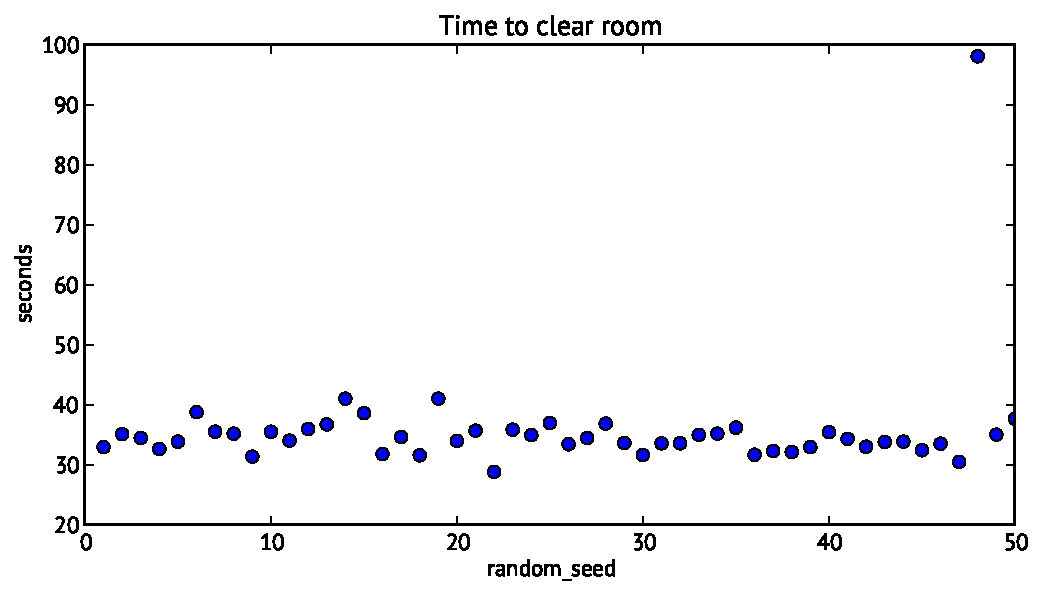
\includegraphics[width=0.8\textwidth]{Figures/random-seed-variations.pdf}
    \caption[Leaving time for different random seeds]{Leaving time for
    different random seeds. Results are dependent on random numbers; for a
    seed value of 48 (top-right corner), one pedestrian starts out walking
    very slowly impacting the total leaving time.}
    \label{fig:random-seed}
\end{figure}


\subsection{Summary}
We have discussed several possible causes for discrepancies in our model, and
possible remedies. The forces in the model only have a repulsive component
that depends on the relative positions but not the relative velocity between
pedestrians.  This could be remedied by adding perpendicular forces and forces
that are dependent on walking speed, which might produce better results.
Depending on the way they are formulated, such forces could be interpreted as
frictional forces between agents. Selection of parameters is also a possible
source of error; a possible remedy, that is inaccessible to us, is obtaining
parameters from real-world experiments, by fitting data to simulations.
Finally, errors arising from the nature of our implementation might occur.
This includes possible coding errors, and errors as a result of extremely
small or large random numbers used when setting initial conditions. This can
be somewhat mitigated by testing the implementation, and by discarding very
small or large random numbers.

In the next section we will assess social force models in a more general
sense, and give our opinion of the state of social force models.
